\input{../utils/preamble}
\createdgmtitle{12}

\usepackage{tikz}

\usetikzlibrary{arrows,shapes,positioning,shadows,trees}
%--------------------------------------------------------------------------------
\begin{document}
%--------------------------------------------------------------------------------
\begin{frame}[noframenumbering,plain]
%\thispagestyle{empty}
\titlepage
\end{frame}
%=======
\begin{frame}{Recap of previous lecture}
	\begin{figure}
		\includegraphics[width=0.8\linewidth]{figs/DDPM}
	\end{figure}
	\vspace{-0.5cm}
	\begin{block}{Reverse process}
		\vspace{-0.5cm}
		{\small
		\[
			q(\bx_{t-1}|\bx_{t}) = \frac{q(\bx_{t}|\bx_{t-1}) {\color{violet}q(\bx_{t-1})}}{{\color{violet}q(\bx_{t})}} \approx p(\bx_{t - 1} | \bx_t, \btheta) = \cN \left(\bmu_{\btheta}(\bx_t, t), \bsigma_{\btheta}^2(\bx_t, t)\right)
		\]
		}
		\vspace{-0.5cm}
	\end{block}
	\begin{minipage}{0.5\linewidth}
		\begin{block}{Forward process}
			\begin{enumerate}
				\item $\bx_0 = \bx \sim \pi(\bx)$;
				\item $\bx_t = \sqrt{1 - \beta_t} \cdot \bx_{t - 1} + \sqrt{\beta_t} \cdot \bepsilon$;
				\item $\bx_T \sim p_{\infty}(\bx) = \cN(0, \bI)$.
			\end{enumerate}
		\end{block}
	\end{minipage}%
	\begin{minipage}{0.55\linewidth}
		\begin{block}{Reverse process}
			\begin{enumerate}
				\item $\bx_T \sim p_{\infty}(\bx) = \cN(0, \bI)$;
				\item $\bx_{t - 1} = \bsigma_{\btheta}(\bx_t, t) \cdot \bepsilon + \bmu_{\btheta}(\bx_t, t)$;
				\item $\bx_0 = \bx \sim \pi(\bx)$;
			\end{enumerate}
		\end{block}
	\end{minipage}
	\textbf{Note:} The forward process does not have any learnable parameters!
	\myfootnotewithlink{https://lilianweng.github.io/posts/2021-07-11-diffusion-models/}{Weng L. What are Diffusion Models?, blog post, 2021}
\end{frame}
%=======
\begin{frame}{Recap of previous lecture}
	\begin{itemize}
		\item $\bz = (\bx_1, \dots, \bx_T)$ is a latent variable.
		\item Variational posterior distribution
		\vspace{-0.2cm}
		\[
			q(\bz | \bx) = q(\bx_1, \dots, \bx_T | \bx_0) = \prod_{t = 1}^T q(\bx_t | \bx_{t - 1}).
		\]
		\vspace{-0.3cm}
		\item Generative distribution and prior
		\vspace{-0.2cm}
		\[
			p(\bx | \bz, \btheta) = p(\bx_0 | \bx_1, \btheta); \quad 
			p(\bz | \btheta) = \prod_{t=2}^T p(\bx_{t - 1} | \bx_t, \btheta) \cdot p(\bx_T)
		\]
	\end{itemize}
	\vspace{-0.2cm}
	\begin{block}{ELBO}
		\vspace{-0.2cm}
		\[
			\log p(\bx | \btheta) \geq \bbE_{q({\color{teal}\bz} | \bx)} \log \frac{p(\bx, {\color{teal}\bz} | \btheta)}{q({\color{teal}\bz} | \bx)} = \cL(q, \btheta) \rightarrow \max_{q, \btheta}
		\]
		\vspace{-0.5cm}
		\begin{multline*}
			\cL(q, \btheta) =  {\color{olive}\bbE_{q(\bx_1 | \bx_0)} \log p(\bx_0 | \bx_1, \btheta)} - {\color{violet}KL\bigl(q(\bx_T | \bx_0) || p(\bx_T)\bigr)} - \\
			- \sum_{t=2}^T  \underbrace{ \bbE_{q(\bx_t | \bx_0)}KL \bigl(q(\bx_{t-1} | \bx_t, \bx_0) || p(\bx_{t - 1} | \bx_t, \btheta )\bigr)}_{\cL_t}
		\end{multline*}
	\end{block}
	\myfootnotewithlink{https://ayandas.me/blog-tut/2021/12/04/diffusion-prob-models.html}{Das A. An introduction to Diffusion Probabilistic Models, blog post, 2021}
\end{frame}
%=======
\begin{frame}{Recap of previous lecture}
	\begin{block}{ELBO of gaussian diffusion model}
		\vspace{-0.7cm}
		\begin{multline*}
			\cL(q, \btheta) =  {\color{olive}\bbE_{q(\bx_1 | \bx_0)} \log p(\bx_0 | \bx_1, \btheta)} - {\color{violet}KL\bigl(q(\bx_T | \bx_0) || p(\bx_T)\bigr)} - \\
			- \sum_{t=2}^T  \underbrace{ \bbE_{q(\bx_t | \bx_0)}KL \bigl(q(\bx_{t-1} | \bx_t, \bx_0) || p(\bx_{t - 1} | \bx_t, \btheta )\bigr)}_{\cL_t}
		\end{multline*}
		\vspace{-1.0cm}
	\end{block}
	\begin{align*}
		q(\bx_{t-1} | \bx_t, \bx_0) &= \cN(\tilde{\bmu}_t(\bx_t, \bx_0), \tilde{\beta}_t \bI), \\
		p(\bx_{t - 1} | \bx_t, \btheta) &= \cN \bigl(\bmu_{\btheta}(\bx_t, t), {\color{violet}\bsigma_{\btheta}^2(\bx_t, t)}\bigr)
	\end{align*}
	Our assumption:	${\color{violet}\bsigma_{\btheta}^2(\bx_t, t) = \tilde{\beta}_t \bI}$.
	\[
		\cL_t = \bbE_{q(\bx_t | \bx_0)} \left[\frac{1}{2\tilde{\beta}_t} \bigl\| \tilde{\bmu}_t(\bx_t, \bx_0) - \bmu_{\btheta}(\bx_t, t) \bigr\|^2  \right]
	\]
	\myfootnotewithlink{https://arxiv.org/abs/2006.11239}{Ho J. Denoising Diffusion Probabilistic Models, 2020}
\end{frame}
%=======
\begin{frame}{Recap of previous lecture}
	\vspace{-0.3cm}
	\[
		\cL_t = \bbE_{\color{violet}q(\bx_t | \bx_0)} \left[ {\color{olive}\frac{1}{2\tilde{\beta}_t}} \bigl\| \tilde{\bmu}_t(\bx_t, \bx_0) - \bmu_{\btheta}(\bx_t, t) \bigr\|^2  \right]
	\]
	\vspace{-0.3cm}
	\begin{block}{Reparametrization}
		\vspace{-0.7cm}
		\begin{align*}
			\tilde{\bmu}_t(\bx_t, \bx_0) &= \frac{1}{\sqrt{\alpha_t}} \cdot \bx_t - \frac{1 - \alpha_t}{\sqrt{\alpha_t (1 - \bar{\alpha}_t)}} \cdot \bepsilon \\
			\bmu_{\btheta}(\bx_t, t) &= \frac{1}{\sqrt{\alpha_t}} \cdot \bx_t - \frac{1 - \alpha_t}{\sqrt{\alpha_t (1 - \bar{\alpha}_t)}} \cdot \bepsilon_{\btheta}({\color{teal}\bx_t}, t)
		\end{align*}
		\vspace{-0.7cm}
	\end{block}
	\vspace{-0.2cm}
	\[
		\cL_t  =	 \bbE_{\color{violet}\bepsilon \sim \cN(0, \bI)} \left[ \frac{(1 - \alpha_t)^2}{2\tilde{\beta}_t \alpha_t (1 - \bar{\alpha}_t)} \Bigl\| \bepsilon - \bepsilon_{\btheta}\bigl( {\color{teal}\sqrt{\bar{\alpha}_t} \bx_0 + \sqrt{1 - \bar{\alpha}_t} \bepsilon}, t\bigr) \Bigr\|^2 \right]
	\]
	At each step of reverse diffusion process we try to predict the noise~$\bepsilon$ that we used in the forward diffusion process!
	\begin{block}{Simplified objective}
		\vspace{-0.7cm}
		\[
			 \cL_{\text{simple}} = \bbE_{t \sim U\{2, T\}} \bbE_{\bepsilon \sim \cN(0, \bI)} \Bigl\| \bepsilon - \bepsilon_{\btheta}\bigl( \sqrt{\bar{\alpha}_t} \bx_0 + \sqrt{1 - \bar{\alpha}_t} \bepsilon, t\bigr) \Bigr\|^2 
		\]
	\end{block}
	\myfootnotewithlink{https://arxiv.org/abs/2006.11239}{Ho J. Denoising Diffusion Probabilistic Models, 2020}
	\end{frame}
%=======
\begin{frame}{Outline}
	\tableofcontents
\end{frame}
%=======
\section{Denoising Diffusion Probabilistic Model (DDPM)}
%=======
\begin{frame}{Generative models zoo}
	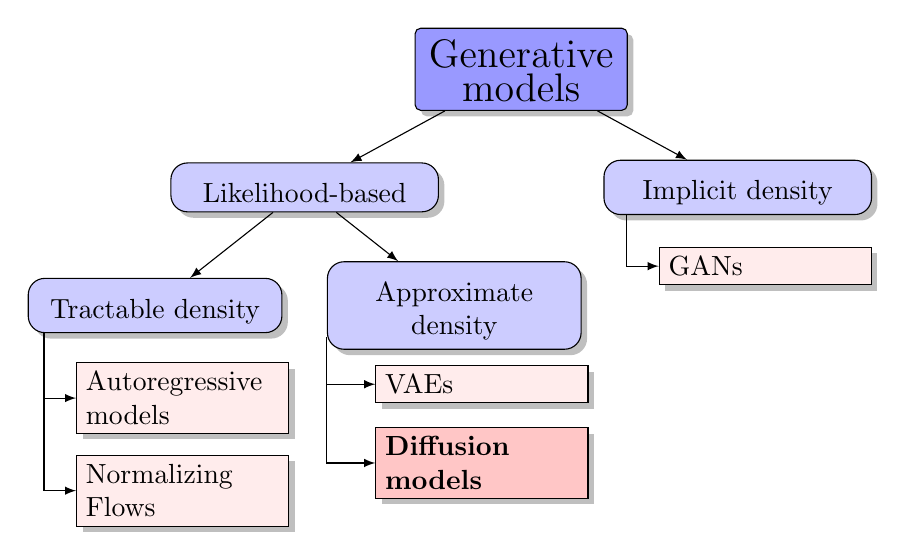
\begin{tikzpicture}[
		basic/.style  = {draw, text width=2cm, drop shadow, rectangle},
		root/.style   = {basic, rounded corners=2pt, thin, text height=1.1em, text width=7em, align=center, fill=blue!40},
		level 1/.style={sibling distance=55mm},
		level 2/.style = {basic, rounded corners=6pt, thin, align=center, fill=blue!20, text height=1.1em, text width=9em, sibling distance=38mm},
		level 3/.style = {basic, rounded corners=6pt, thin,align=center, fill=blue!20, text width=8.5em},
		level 4/.style = {basic, thin, align=left, fill=pink!30, text width=7em},
		level 5/.style = {basic, thin, align=left, fill=pink!90, text width=7em},
		edge from parent/.style={->,draw},
		>=latex]
		
		% root of the the initial tree, level 1
		\node[root] {\Large Generative models}
		% The first level, as children of the initial tree
		child {node[level 2] (c1) {Likelihood-based}
			child {node[level 3] (c11) {Tractable density}}
			child {node[level 3] (c12) {Approximate density}}
		}
		child {node[level 2] (c2) {Implicit density}};
		
		% The second level, relatively positioned nodes
		\begin{scope}[every node/.style={level 4}]
			\node [below of = c11, yshift=-5pt, xshift=10pt] (c111) {Autoregressive models};
			\node [below of = c111, yshift=-5pt] (c112) {Normalizing Flows};
			\node [below of = c12, xshift=10pt] (c121) {VAEs};
			
			\node [below of = c2, xshift=10pt] (c21) {GANs};
		\end{scope}
		
		% The second level, relatively positioned nodes
		\begin{scope}[every node/.style={level 5}]
			\node [below of = c121] (c122) {\textbf{Diffusion \\ models}};
		\end{scope}
		
		% lines from each level 1 node to every one of its "children"
		\foreach \value in {1,2}
		\draw[->] (c11.194) |- (c11\value.west);
		
		\foreach \value in {1,2}
		\draw[->] (c12.194) |- (c12\value.west);
		
		\draw[->] (c2.194) |- (c21.west);
		
	\end{tikzpicture}
\end{frame}
%=======
\begin{frame}{Denoising diffusion probabilistic model (DDPM)}
	\begin{block}{DDPM is a VAE model}
		\begin{itemize}
			\item Encoder is a fixed Gaussian Markov chain $q(\bx_1, \dots, \bx_T | \bx_0)$.
			\item Latent variable is a hierarchical (in each step the dim. of the latent equals to the dim of the input).
			\item Decoder is a simple Gaussian model $p(\bx_0 | \bx_1, \btheta)$.
			\item Prior distribution is given by parametric Gaussian Makov chain $p(\bx_{t-1} | \bx_t, \btheta)$.
		\end{itemize}
	\end{block}
	\begin{minipage}{0.5\linewidth}
		\begin{block}{Forward process}
			\begin{enumerate}
				\item $\bx_0 = \bx \sim \pi(\bx)$;
				\item $\bx_t = \sqrt{1 - \beta_t} \cdot \bx_{t - 1} + \sqrt{\beta_t} \cdot \bepsilon$;
				\item $\bx_T \sim p_{\infty}(\bx) = \cN(0, \bI)$.
			\end{enumerate}
		\end{block}
	\end{minipage}%
	\begin{minipage}{0.55\linewidth}
		\begin{block}{Reverse process}
			\begin{enumerate}
				\item $\bx_T \sim p_{\infty}(\bx) = \cN(0, \bI)$;
				\item $\bx_{t - 1} = \bsigma_{\btheta}(\bx_t, t) \cdot \bepsilon + \bmu_{\btheta}(\bx_t, t)$;
				\item $\bx_0 = \bx \sim \pi(\bx)$;
			\end{enumerate}
		\end{block}
	\end{minipage}
	\myfootnotewithlink{https://arxiv.org/abs/2006.11239}{Ho J. Denoising Diffusion Probabilistic Models, 2020}
\end{frame}
%=======
\begin{frame}{Denoising diffusion probabilistic model (DDPM)}
	\begin{block}{Training}
		\begin{enumerate}
			\item Get the sample $\bx_0 \sim \pi(\bx)$.
			\item Sample timestamp $t \sim U\{1, T\}$ and the noise $\bepsilon \sim \cN(0, \bI)$.
			\item Get noisy image $\bx_t = \sqrt{\bar{\alpha}_t} \cdot \bx_0 + \sqrt{1 - \bar{\alpha}_t} \cdot \bepsilon$.
			\item Compute loss $ \cL_{\text{simple}} = \| \bepsilon - \bepsilon_{\btheta}(\bx_t , t) \|^2 $.
		\end{enumerate}
	\end{block}
	\begin{block}{Sampling}
		\begin{enumerate}
			\item Sample $\bx_T \sim \cN(0, \bI)$.
			\item Compute mean of $p(\bx_{t-1} | \bx_t, \btheta) = \cN(\bmu_{\btheta}(\bx_t, t), \tilde{\beta}_t \bI)$:
			\[
				\bmu_{\btheta}(\bx_t, t) = \frac{1}{\sqrt{\alpha_t}} \cdot \bx_t - \frac{1 - \alpha_t}{\sqrt{\alpha_t (1 - \bar{\alpha}_t)}} \cdot \bepsilon_{\btheta}(\bx_t, t)
			\]
			\vspace{-0.3cm}
			\item Get denoised image $\bx_{t - 1} = \bmu_{\btheta}(\bx_t, t) +  \sqrt{\tilde{\beta}_t} \cdot \bepsilon$, where $\bepsilon \sim \cN(0, \bI)$.
		\end{enumerate}
	\end{block}
	\myfootnotewithlink{https://arxiv.org/abs/2006.11239}{Ho J. Denoising Diffusion Probabilistic Models, 2020}
\end{frame}
%=======
\begin{frame}{Denoising diffusion probabilistic model (DDPM)}
	\begin{block}{Samples}
		\begin{figure}
			\includegraphics[width=\linewidth]{figs/ddpm_samples}
		\end{figure}
	\end{block}
	\myfootnotewithlink{https://arxiv.org/abs/2006.11239}{Ho J. Denoising Diffusion Probabilistic Models, 2020}
\end{frame}
%=======
\section{Denosing diffusion as score-based generative model}
%=======
\begin{frame}{Denosing diffusion as score-based generative model}
	\begin{block}{DDPM objective}
		\vspace{-0.5cm}
		\[
			\cL_t = \bbE_{\bepsilon \sim \cN(0, \bI)} \left[ \frac{(1 - \alpha_t)^2}{2\tilde{\beta}_t \alpha_t  {\color{teal}(1 - \bar{\alpha}_t)}}  \Bigl\|  \bepsilon_{\btheta}\bigl( \sqrt{\bar{\alpha}_t} \bx_0 + \sqrt{1 - \bar{\alpha}_t} \bepsilon, t\bigr) {\color{teal} - \bepsilon}\Bigr\|_2^2  \right]
		\]
		\vspace{-0.7cm}
	\end{block}
	\vspace{-0.5cm}
	\begin{align*}
		q(\bx_t | \bx_0) &= \cN(\sqrt{\bar{\alpha}_t} \cdot \bx_0, (1 - \bar{\alpha}_t) \cdot \bI) \\
		\nabla_{\bx_t} \log q(\bx_t | \bx_0) &= - \frac{\bx_t - \sqrt{\bar{\alpha}_t} \cdot \bx_0}{1 - \bar{\alpha}_t} = {\color{teal}-  \frac{\bepsilon}{\sqrt{1 - \bar{\alpha}_t}}}.
	\end{align*}
		Let reparametrize our model: 
		\vspace{-0.2cm}
		\[
			\bs_{\btheta}(\bx_t, t) = - \frac{\bepsilon_{\btheta}(\bx_t, t)}{\sqrt{1 - \bar{\alpha}_t}}.
		\]
		\[
			\cL_t = \bbE_{q(\bx_t | \bx_0)} \left[ \frac{(1 - \alpha_t)^2}{2\tilde{\beta}_t \alpha_t}  \Bigl\|  \bs_{\btheta} (\bx_t, t) - \nabla_{\bx_t} \log q(\bx_t | \bx_0) \Bigr\|_2^2  \right]
		\]
	\myfootnotewithlink{https://arxiv.org/abs/2006.11239}{Ho J. Denoising Diffusion Probabilistic Models, 2020}
	\end{frame}
%=======
\begin{frame}{Denosing diffusion as score-based generative model}
	\begin{block}{DDPM objective}
		\vspace{-0.5cm}
		\[
			\bbE_{\pi(\bx_0)} \bbE_{t \sim U\{1, T\}}\bbE_{q(\bx_t | \bx_0)} \left[ {\color{olive}\frac{(1 - \alpha_t)^2}{2\tilde{\beta}_t \alpha_t}} \Bigl\|  \bs_{\btheta} (\bx_t, t) - \nabla_{\bx_t} \log q(\bx_t | \bx_0) \Bigr\|_2^2  \right]
		\]
		In practice {\color{olive}the coefficient} is omitted.
	\end{block}
	\begin{block}{NCSN objective}
		\vspace{-0.3cm}
		\[
			\bbE_{\pi(\bx_0)} \bbE_{t \sim U\{1, T\}} \bbE_{q(\bx_t | \bx_0)}\bigl\| \bs_{\btheta, \sigma_t}(\bx_t) - \nabla_{\bx_t} \log q(\bx_t | \bx_0) \bigr\|^2_2 
		\]
		\vspace{-0.3cm}
	\end{block}
	\textbf{Note:} The objective of DDPM and NCSN is almost identical. But the difference in sampling scheme:
	\begin{itemize}
		\item NCSN uses annealed Langevin dynamics;
		\item DDPM uses ancestral sampling.
	\end{itemize}
	\myfootnotewithlink{https://arxiv.org/abs/2006.11239}{Ho J. Denoising Diffusion Probabilistic Models, 2020}
	\end{frame}
%=======
\section{Guidance}
%=======
\begin{frame}{Guidance}
	\begin{itemize}
	\item Throughout the whole course we have discussed unconditional generative models $p(\bx | \btheta)$.
	\item In practice the majority of the generative models are $\textbf{conditional}$: $p(\bx | \by, \btheta)$.
	\item Here $\by$ could be the class label or $\textbf{text}$ (for text-to-image models).
	\end{itemize}
	\vspace{-0.3cm}
	\begin{minipage}[t]{0.5\columnwidth}
		\begin{figure}
			\includegraphics[width=0.9\linewidth]{figs/shedevrum1}
		\end{figure}
	\end{minipage}%
	\begin{minipage}[t]{0.5\columnwidth}
		\begin{figure}
			\includegraphics[width=0.9\linewidth]{figs/shedevrum2}
		\end{figure}
	\end{minipage}
\end{frame}
%=======
\begin{frame}{Guidance}
	\begin{block}{How to make conditional model $p(\bx | \by, \btheta)$?}
		\begin{itemize}
		\item If we have \textbf{supervised} data $\{(\bx_i, \by_i)\}_{i=1}^m$ we could theat $\by$ as additional model input:
		\begin{itemize}
			\item $p(x_j | \bx_{1:j-1}, {\color{olive}\by}, \btheta)$ for AR;
			\item Encoder $q(\bz | \bx, {\color{olive}\by}, \bphi)$ and decoder $p(\bx | \bz, {\color{olive}\by}, \btheta)$ for VAE;
			\item $G_{\btheta}(\bz, {\color{olive}\by})$ for NF and GAN;
			\item $p(\bx_{t-1} | \bx_t, {\color{olive}\by}, \btheta)$ for DDPM.
		\end{itemize}
		\item If we have \textbf{unsupervised} data $\{\bx_i\}_{i=1}^m$ we need to create the way to convert unconditional model $p(\bx | \btheta)$ to the conditional.
		\end{itemize}
	\end{block}
	\begin{block}{DDPM \textbf{unsupervised} guidance}
		\begin{itemize}
			\item Let imagine we are given the distribution $q(\by | \bx_0)$. 
			\item Since we have already defined Markov chain, we have $q(\bx_t | \bx_{t-1}, \by) = q(\bx_t | \bx_{t - 1})$.
			\item Let try to find reverse $q(\bx_{t-1} | \bx_t, \by)$.
		\end{itemize}
	\end{block}
\end{frame}
%=======
\begin{frame}{Label guidance}
	\textbf{Label:} Ostrich (10th ImageNet class) 
	\begin{figure}
		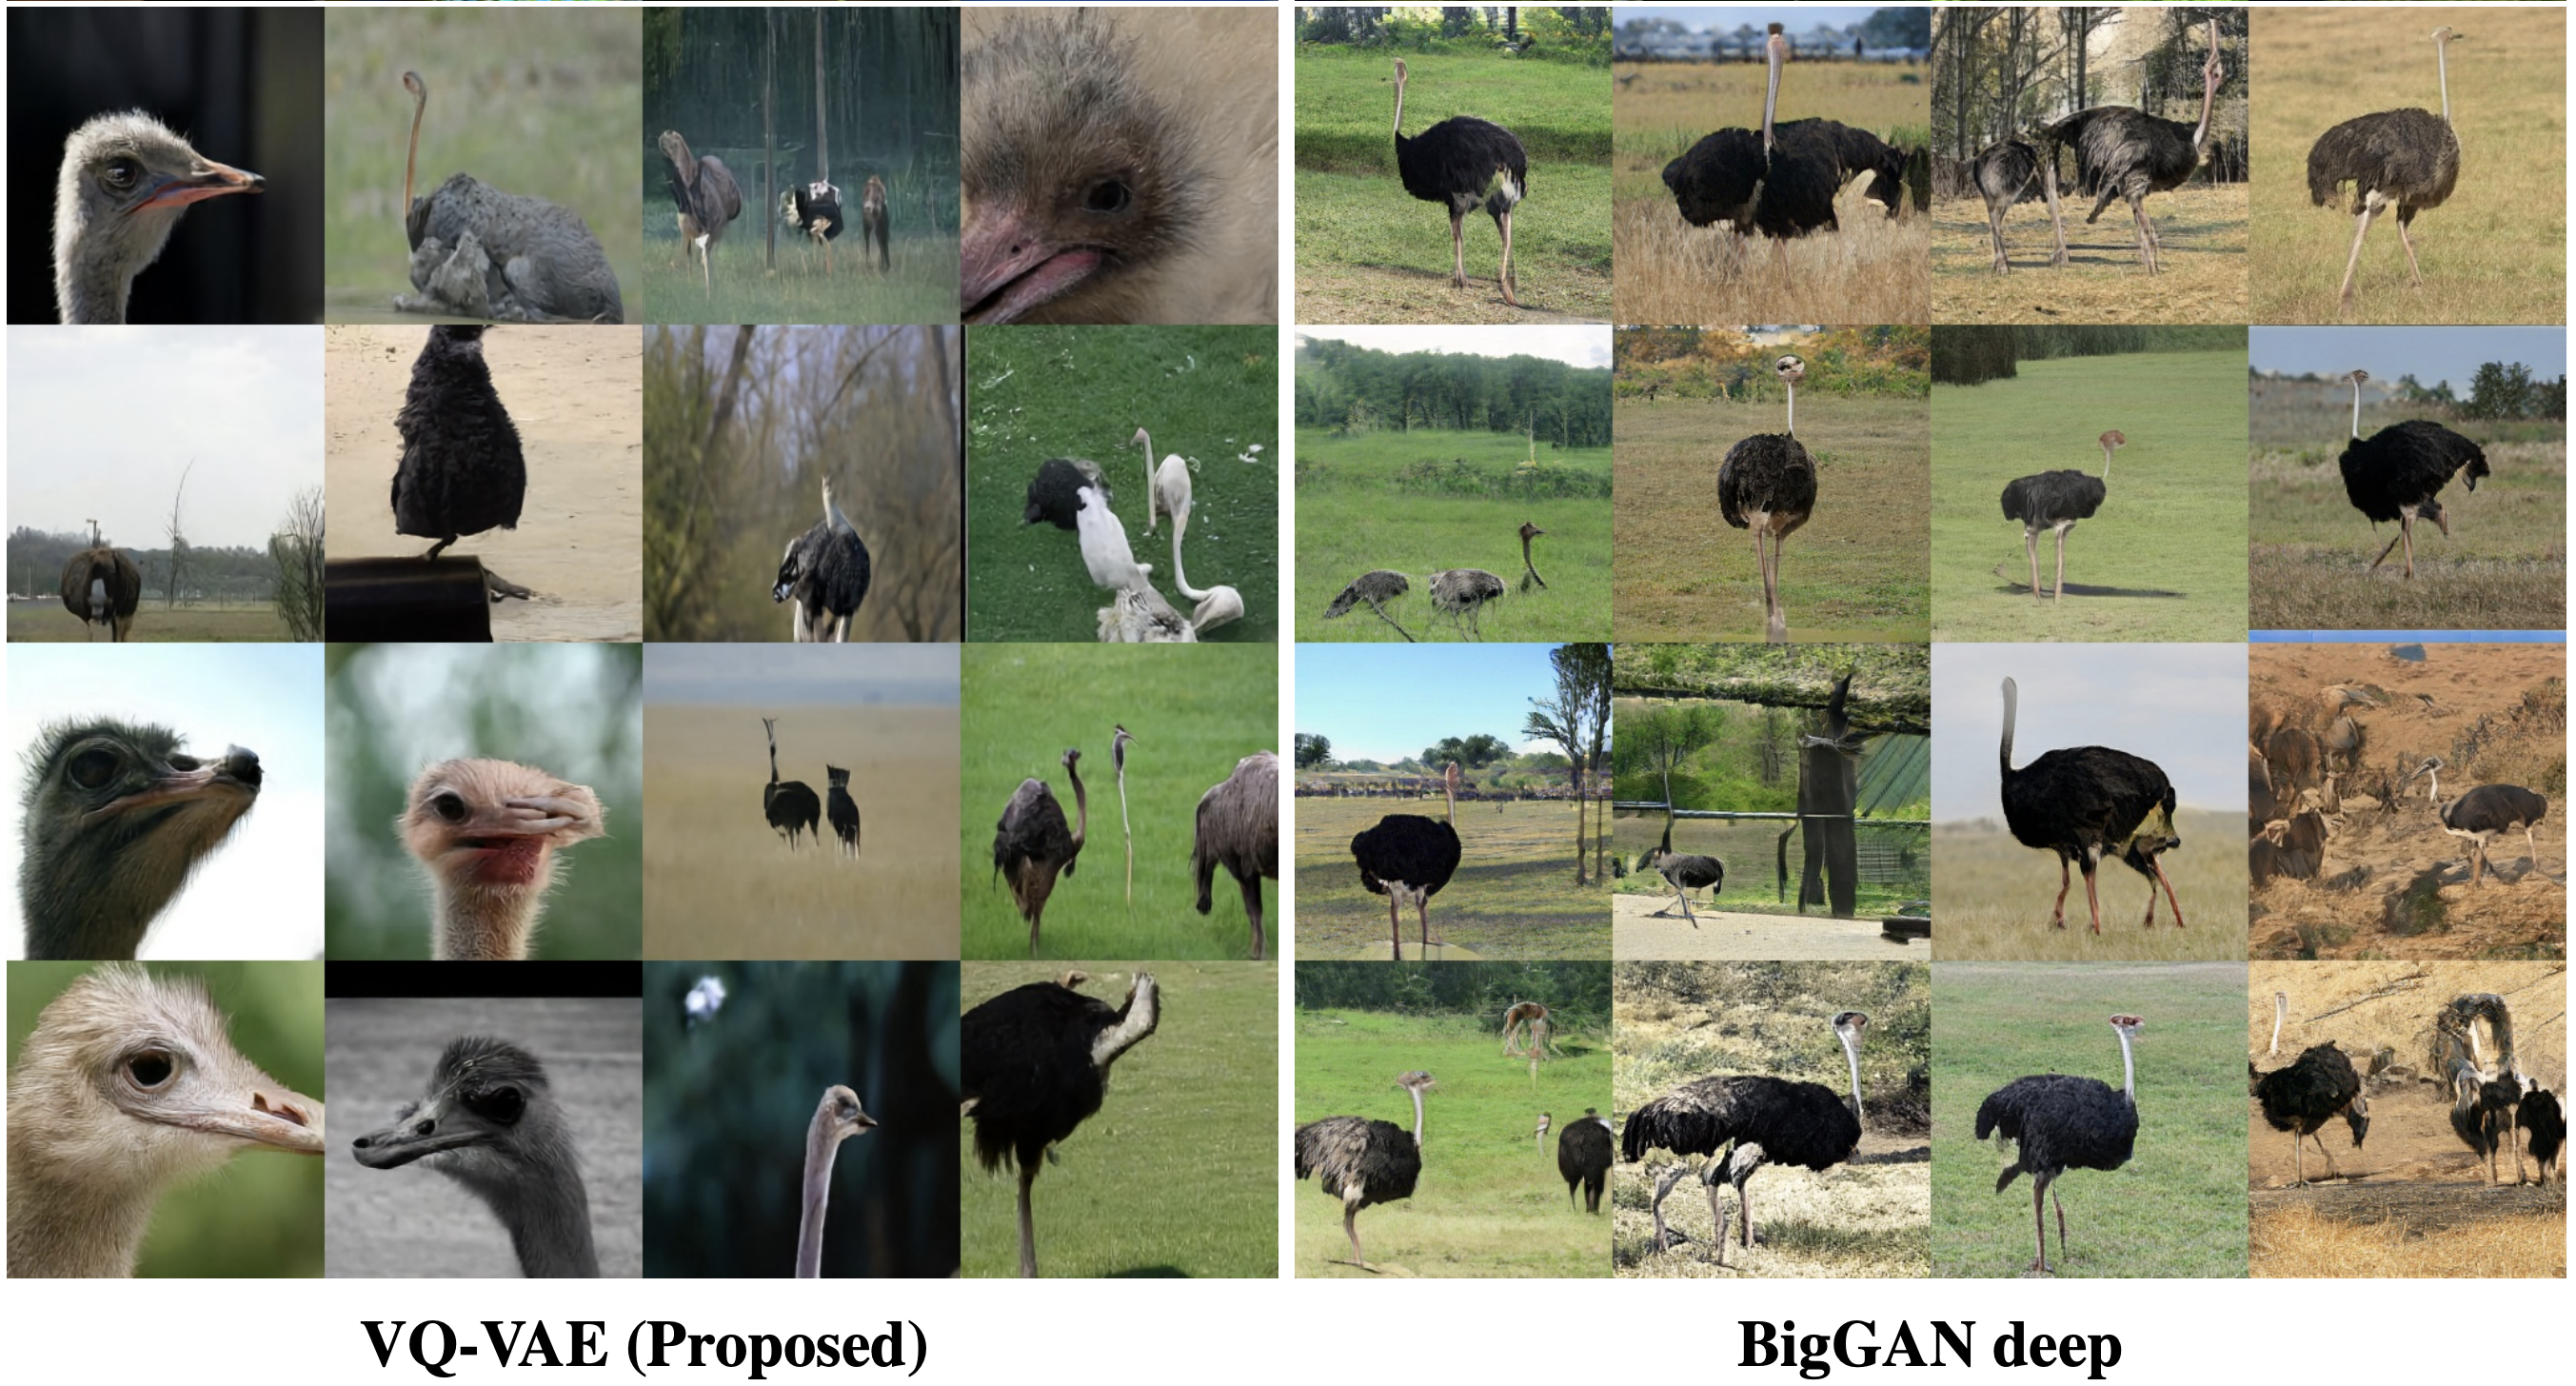
\includegraphics[width=\linewidth]{figs/label_conditioning}
	\end{figure}
	\myfootnotewithlink{https://arxiv.org/abs/1906.00446}{Razavi A., Oord A., et al. Generating Diverse High-Fidelity Images with VQ-VAE-2, 2019}\end{frame}
%=======
\begin{frame}{Text guidance}
	\textbf{Prompt:} a stained glass window of a panda eating bamboo \\
	Left: $\gamma = 1$, Right: $\gamma = 3$.
	\begin{figure}
		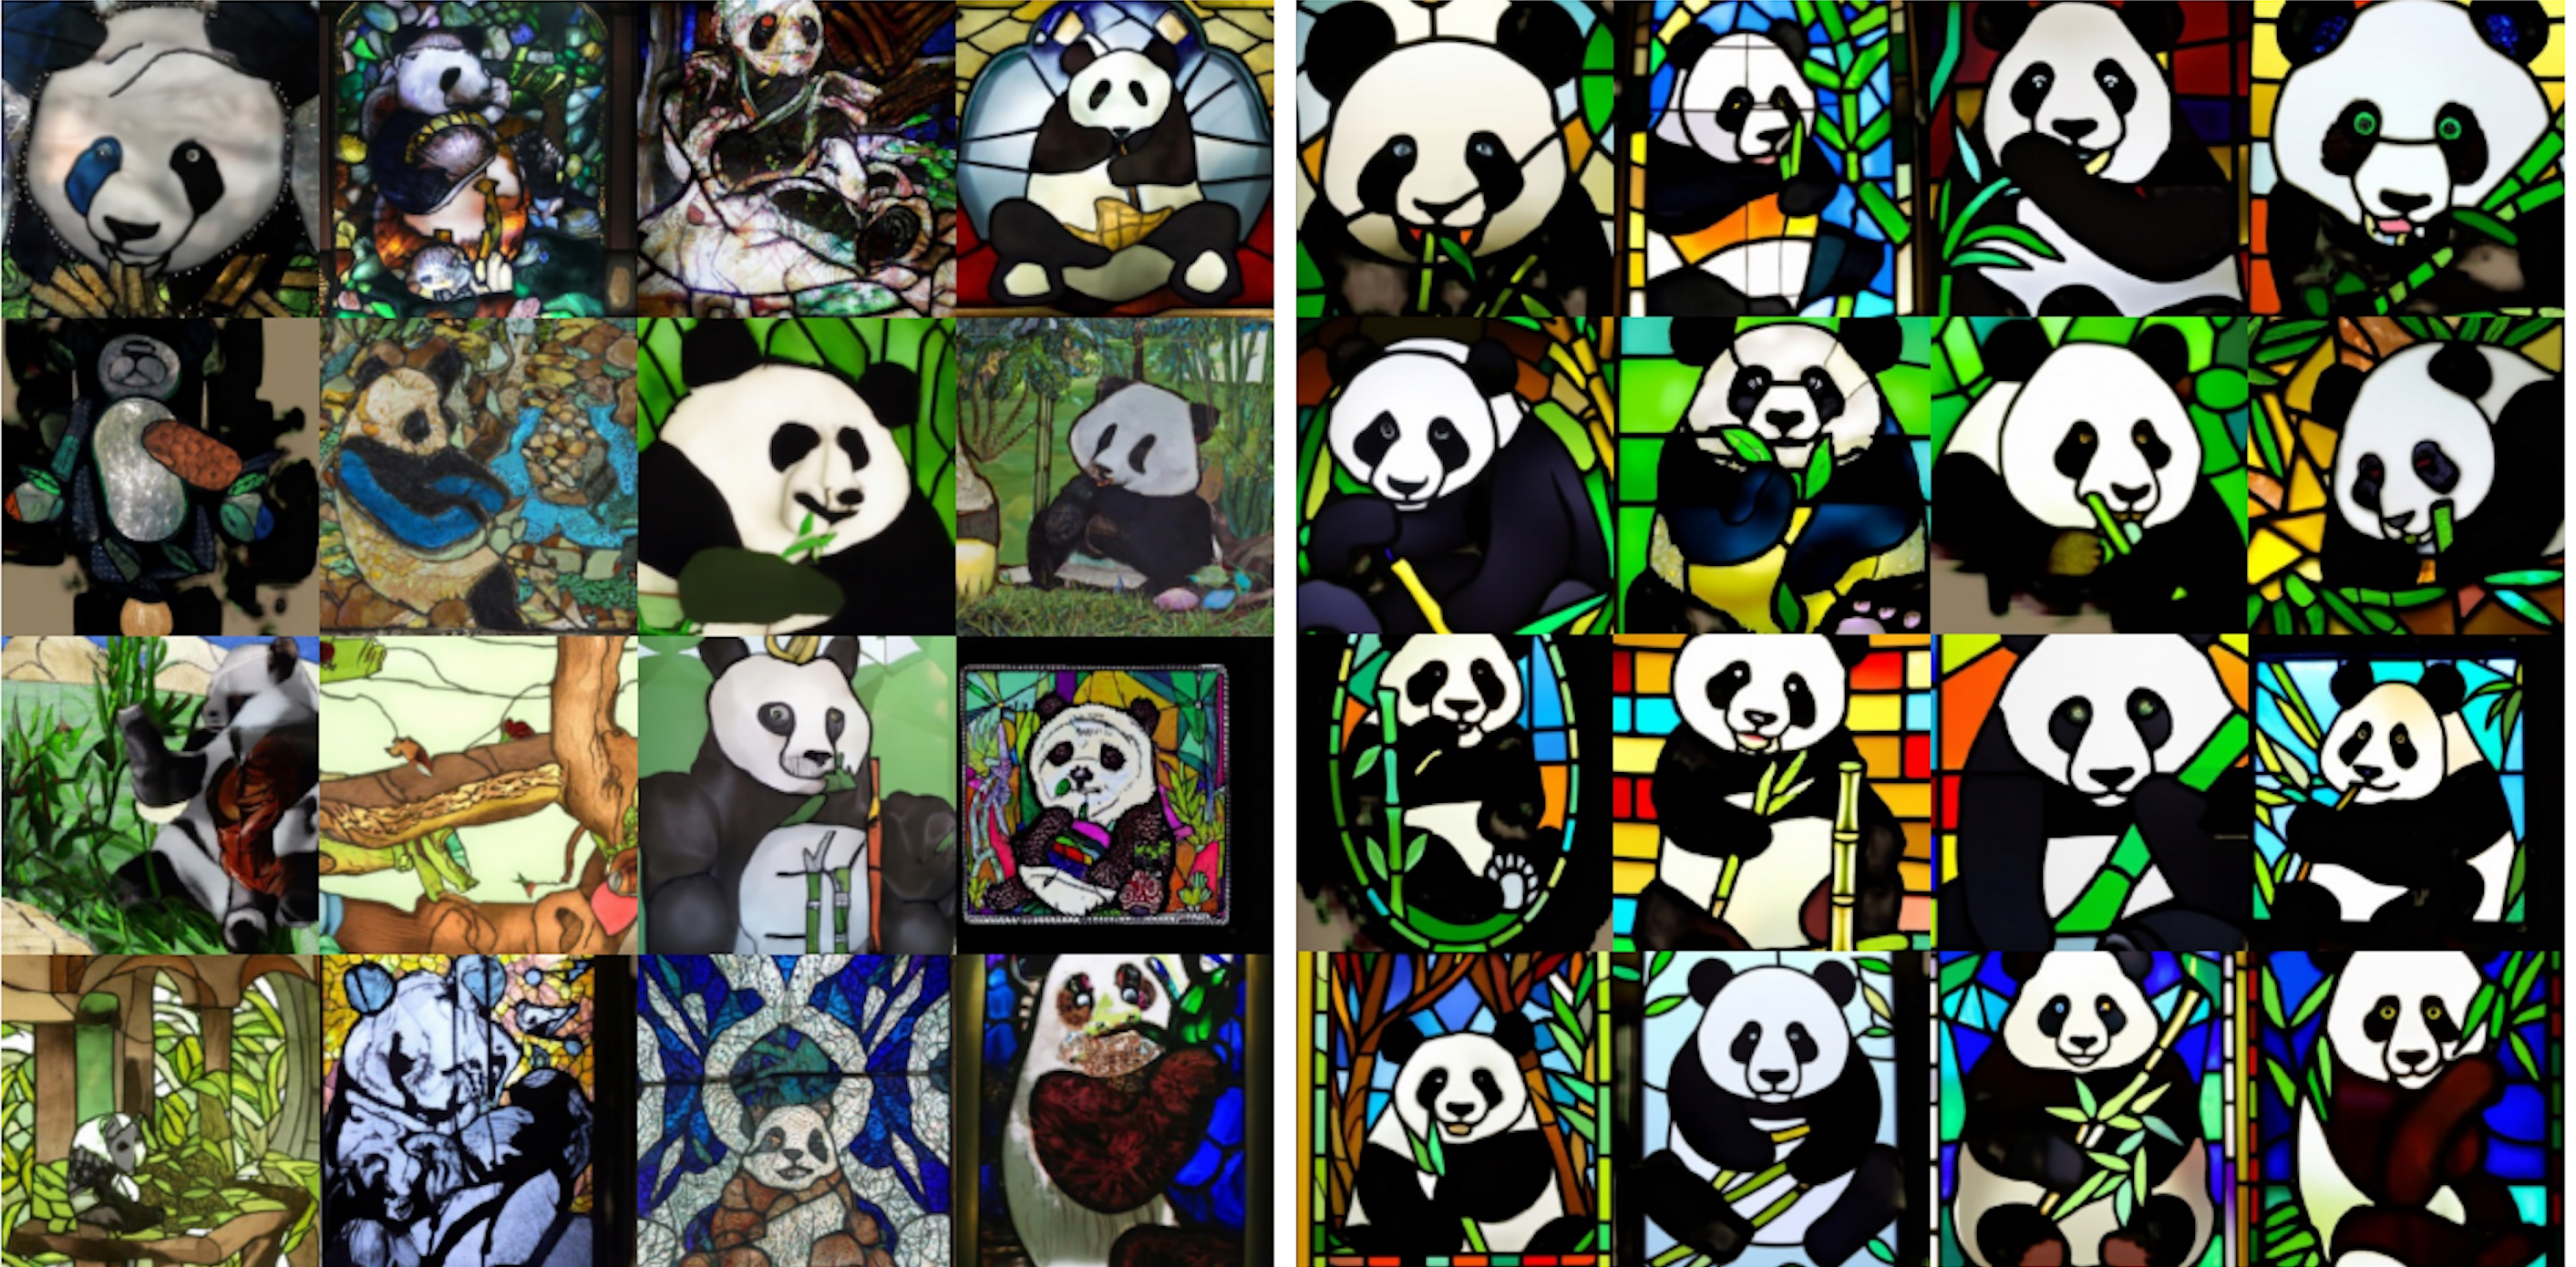
\includegraphics[width=\linewidth]{figs/cfg}
	\end{figure}
	\myfootnotewithlink{https://arxiv.org/pdf/2112.10741}{Nichol A., et al. GLIDE: Towards Photorealistic Image Generation and Editing with Text-Guided Diffusion Models, 2022}
\end{frame}
%=======
\subsection{Classifier guidance}
%=======
\begin{frame}{Classifier guidance}
	\vspace{-0.5cm}
	\begin{multline*}
		{\color{teal}q(\by | \bx_{t - 1}, \bx_t)} = \frac{q(\bx_{t - 1}, \bx_t, \by)}{q(\bx_{t - 1}, \bx_t)} = \\
		= \frac{q(\bx_t | \bx_{t - 1}, {\color{olive}\by}) q(\by | \bx_{t - 1}) \color{violet}{q(\bx_{t - 1})}} {q(\bx_t | \bx_{t - 1}) \color{violet}{q(\bx_{t - 1})}} = q(\by | \bx_{t - 1}).
	\end{multline*}
	\vspace{-0.4cm}
	\begin{block}{Conditional distribution}
		\vspace{-0.7cm}
		\begin{multline*}
			q(\bx_{t - 1} | \bx_t, \by) = \frac{q(\bx_{t - 1}, \bx_t, \by)}{q(\bx_t, \by)}  = \\ 
			=  \frac{{\color{teal}q(\by | \bx_{t - 1}, \bx_t)} q(\bx_{t - 1} | \bx_t) {\color{violet}q(\bx_t)}}{q(\by | \bx_t) {\color{violet}q(\bx_t)}} = \\
			= q(\by | \bx_{t - 1}) q(\bx_{t - 1} | \bx_t) \cdot \text{const}(\bx_{t - 1}).
		\end{multline*}
		\[
			p(\bx_{t - 1} | \bx_t, \by, \btheta , \bphi) = p(\by | \bx_{t-1}, \bphi) p(\bx_{t-1} | \bx_t, \btheta) \cdot \text{const}(\bx_{t - 1}).
		\]
		\vspace{-0.4cm}
		\begin{itemize}
			\item $p(\bx_{t-1} | \bx_t, \btheta)$ - our unsupervised diffusion model.
			\item $p(\by | \bx_{t-1}, \bphi)$ - classifier for noised samples $\bx_{t-1}$
		\end{itemize}
	\end{block}
	\myfootnotewithlink{https://arxiv.org/abs/2105.05233}{Dhariwal P., Nichol A. Diffusion Models Beat GANs on Image Synthesis, 2021}
\end{frame}
%=======
\begin{frame}{Classifier guidance}
	\begin{block}{Conditional distribution}
		\vspace{-0.5cm}
		\begin{align*}
			p(\bx_{t - 1} | \bx_t, \by, \btheta , \bphi) &= p(\by | \bx_{t-1}, \bphi) \cdot p(\bx_{t-1} | \bx_t, \btheta) \cdot \text{const}(\bx_{t - 1}) \\
			\log p(\bx_{t - 1} | \bx_t, \by, \btheta , \bphi) &= {\color{teal}\log p(\by | \bx_{t-1}, \bphi)} + {\color{violet}\log p(\bx_{t-1} | \bx_t, \btheta)} + \text{const}
		\end{align*}
	\end{block}
	\vspace{-0.7cm}
	\begin{align*}
		p(\bx_{t-1} | \bx_t, \btheta) &= \cN(\bmu_{\btheta}(\bx_t, t), \bsigma^2_{\btheta}(\bx_t, t)) \\
		{\color{violet}\log p(\bx_{t-1} | \bx_t, \btheta)} &= - \frac{\|\bx_{t - 1} - \bmu\|^2}{2 \bsigma^2} + \text{const}(\bx_{t-1})
	\end{align*}
	\vspace{-0.5cm}
	\begin{block}{Taylor expansion}
		\vspace{-0.7cm}
		\begin{multline*}
			{\color{teal}\log p(\by | \bx_{t-1}, \bphi)} \approx \log p(\by | \bx_{t-1}, \bphi) |_{\bx_{t-1} = \bmu} + \\
			+ (\bx_{t-1} - \bmu) \cdot \nabla_{\bx_{t-1}} \log p(\by | \bx_{t-1}, \bphi) |_{\bx_{t-1} = \bmu} = \\
			= (\bx_{t-1} - \bmu) \cdot \mathbf{g} +  \text{const}(\bx_{t-1}),
		\end{multline*}
		where $\mathbf{g} =  \nabla_{\bx_{t-1}} \log p(\by | \bx_{t-1}, \bphi) |_{\bx_{t-1} = \bmu}$.
	\end{block}
	\myfootnotewithlink{https://arxiv.org/abs/2105.05233}{Dhariwal P., Nichol A. Diffusion Models Beat GANs on Image Synthesis, 2021}
\end{frame}
%=======
\begin{frame}{Classifier guidance}
	\vspace{-0.5cm}
	\begin{align*}
		\log p(\bx_{t - 1} | \bx_t, \by, \btheta , \bphi) &= {\color{teal}(\bx_{t-1} - \bmu) \cdot \mathbf{g}} - {\color{violet}\frac{\|\bx_{t - 1} - \bmu\|^2}{2 \bsigma^2}} + \text{const}(\bx_{t-1}) \\
		& = - \frac{\|\bx_{t - 1} - \bmu - \bsigma \odot \mathbf{g}\|^2}{2 \bsigma^2} + \text{const}(\bx_{t-1}) \\
		& = \log \cN( \bmu + {\color{olive}\bsigma \odot \mathbf{g}}, \bsigma^2) + \text{const}(\bx_{t-1})
	\end{align*}
	\vspace{-0.5cm}
	\begin{block}{Guided sampling}
		\begin{enumerate}
			\item Sample $\bx_T \sim \cN(0, \bI)$.
			\item Compute mean of $p(\bx_{t-1} | \bx_t, \btheta) = \cN(\bmu_{\btheta}(\bx_t, t), \tilde{\beta}_t \bI)$:
			\[
				\bmu_{\btheta}(\bx_t, t) = \frac{1}{\sqrt{\alpha_t}} \bx_t - \frac{1 - \alpha_t}{\sqrt{\alpha_t (1 - \bar{\alpha}_t)}} \cdot \bepsilon_{\btheta}(\bx_t, t).
			\]
			\vspace{-0.3cm}
			\item Compute $\mathbf{g} =  \nabla_{\bx_{t-1}} \log p(\by | \bx_{t-1}, \bphi) |_{\bx_{t-1} = \bmu}$.
			\item Get denoised image $\bx_{t - 1} = (\bmu_{\btheta}(\bx_t, t) +  {\color{olive} \sqrt{\tilde{\beta}_t} \cdot \mathbf{g}})+ \sqrt{\tilde{\beta}_t} \cdot \bepsilon$, where $\bepsilon \sim \cN(0, \bI)$.
		\end{enumerate}
	\end{block}
	\myfootnotewithlink{https://arxiv.org/abs/2105.05233}{Dhariwal P., Nichol A. Diffusion Models Beat GANs on Image Synthesis, 2021}
\end{frame}
%=======
\begin{frame}{Classifier guidance}
	\begin{block}{Theorem (denoising score matching)}
		\vspace{-0.8cm}
		\begin{multline*}
			\bbE_{q(\bx_{t})}\bigl\| \bs_{\btheta}(\bx_t, t) - \nabla_{\bx_t} \log q(\bx_t) \bigr\|^2_2 = \\ = \bbE_{\pi(\bx_0)} \bbE_{q(\bx_t | \bx_0)}\bigl\| \bs_{\btheta}(\bx_t, t) - \nabla_{\bx_t} \log q(\bx_t | \bx_0) \bigr\|^2_2 + \text{const}(\btheta)
		\end{multline*}
		\vspace{-1.0cm}
	\end{block}
	\[
		\nabla_{\bx_t} \log p(\bx_t | \btheta) \approx - \frac{\bepsilon_{\btheta}(\bx_t, t)}{\sqrt{1 - \bar{\alpha}_t}} = \bs_{\btheta}(\bx_t, t).
	\]
	\vspace{-0.4cm}
	\begin{block}{Conditional distribution}
		\vspace{-0.7cm}
		\begin{align*}
			{\color{olive}\nabla_{\bx_t} \log p(\bx_t | \by, \btheta, \bphi)} &= \nabla_{\bx_t} \log \left(\frac{p(\by | \bx_t, \bphi)p(\bx_t | \btheta)}{p(\by | \bphi)} \right)\\
			&= \nabla_{\bx_t} \log p(\by | \bx_t, \bphi) + {\color{violet}\nabla_{\bx_t} \log p(\bx_t | \btheta)}\\
			&= {\color{teal}\nabla_{\bx_t} \log p(\by | \bx_t, \bphi)} {\color{violet}- \frac{\bepsilon_{\btheta}(\bx_t, t)}{\sqrt{1 - \bar{\alpha}_t}}}
		\end{align*}
		\vspace{-0.7cm}
	\end{block}
	\begin{block}{Classifier-corrected noise prediction}
		\vspace{-0.4cm}
		\[
			{\color{olive}\hat{\bepsilon}_{\btheta}(\bx_t, t)} = {\color{violet}\bepsilon_{\btheta}(\bx_t, t)} - {\color{violet}\sqrt{1 - \bar{\alpha}_t}} \cdot {\color{teal}\nabla_{\bx_t} \log p(\by | \bx_t, \bphi)}
		\]
	\end{block}
	\myfootnotewithlink{https://arxiv.org/abs/2105.05233}{Dhariwal P., Nichol A. Diffusion Models Beat GANs on Image Synthesis, 2021}
\end{frame}
%=======
\begin{frame}{Classifier guidance}
	\begin{block}{Classifier-corrected noise prediction}
		\vspace{-0.7cm}
		\begin{align*}
			\hat{\bepsilon}_{\btheta}(\bx_t, t) &= \bepsilon_{\btheta}(\bx_t, t) - \sqrt{1 - \bar{\alpha}_t} \cdot \nabla_{\bx_t} \log p(\by | \bx_t, \bphi) \\
			\hat{\bepsilon}_{\btheta}(\bx_t, t) &= \bepsilon_{\btheta}(\bx_t, t) - {\color{teal}\gamma} \cdot \sqrt{1 - \bar{\alpha}_t} \cdot \nabla_{\bx_t} \log p(\by | \bx_t, \bphi)
		\end{align*}
		\vspace{-0.7cm}
	\end{block}
	Here we introduce {\color{teal} guidance scale $\gamma$} that controls the magnitude of the classifier guidance.
	\begin{block}{Conditional distribution}
		\vspace{-0.2cm}
		\[
			\frac{\hat{\bepsilon}_{\btheta}(\bx_t, t)}{\sqrt{1 - \bar{\alpha}_t}} = \frac{\bepsilon_{\btheta}(\bx_t, t)}{\sqrt{1 - \bar{\alpha}_t}} - {\color{teal}\gamma} \cdot \nabla_{\bx_t} \log p(\by | \bx_t, \bphi)
		\]
		\vspace{-0.5cm}
		\begin{align*}
			\nabla_{\bx_t}^{\gamma} \log p(\bx_t | \by, \btheta, \bphi) &= \gamma \cdot \nabla_{\bx_t} \log p(\by | \bx_t, \bphi) + \nabla_{\bx_t} \log p(\bx_t | \btheta) \\
			p(\bx_t | \by, \btheta, \bphi) &= \frac{p(\by | \bx_t, \bphi)^{\gamma} p(\bx_t | \btheta)}{Z}
		\end{align*}
		\vspace{-0.5cm}
	\end{block}
	Check that $\nabla_{\bx_t} \log Z \neq 0$.
	\myfootnotewithlink{https://arxiv.org/abs/2105.05233}{Dhariwal P., Nichol A. Diffusion Models Beat GANs on Image Synthesis, 2021}
\end{frame}
%=======
\begin{frame}{Classifier guidance}
	\begin{block}{Guided sampling}
		\begin{enumerate}
			\item Sample $\bx_T \sim \cN(0, \bI)$.
			\item Compute "corrected" $\hat{\bepsilon}_{\btheta}(\bx_t, t)$:
			\[
				{\color{olive}\hat{\bepsilon}_{\btheta}(\bx_t, t)} = \bepsilon_{\btheta}(\bx_t, t) - {\color{teal}\gamma} \cdot \sqrt{1 - \bar{\alpha}_t} \cdot \nabla_{\bx_t} \log p(\by | \bx_t, \bphi)
			\]
			\item Compute mean of $p(\bx_{t-1} | \bx_t, \btheta) = \cN(\bmu_{\btheta}(\bx_t, t), \tilde{\beta}_t \bI)$:
			\[
				\bmu_{\btheta}(\bx_t, t) = \frac{1}{\sqrt{\alpha_t}} \bx_t - \frac{1 - \alpha_t}{\sqrt{\alpha_t (1 - \bar{\alpha}_t)}} \cdot  	{\color{olive}\hat{\bepsilon}_{\btheta}(\bx_t, t)}
			\]
			\vspace{-0.3cm}
			\item Get denoised image $\bx_{t - 1} = \bmu_{\btheta}(\bx_t, t) +  \sqrt{\tilde{\beta}_t} \cdot \bepsilon$, where $\bepsilon \sim \cN(0, \bI)$.
		\end{enumerate}
	\end{block}
	\myfootnotewithlink{https://arxiv.org/abs/2105.05233}{Dhariwal P., Nichol A. Diffusion Models Beat GANs on Image Synthesis, 2021}
\end{frame}
%=======
\subsection{Classifier-free guidance}
%=======
\begin{frame}{Classifier-free guidance}
	Previous methods require training the additional classifier model $p(\by | \bx_t, \btheta)$ on the noisy data.
	Let try to avoid this requirement.
	\vspace{-0.3cm}
	\begin{multline*}
		\nabla_{\bx_t}^{\gamma} \log p(\bx_t | \by, \btheta, \bphi) = \gamma \cdot \nabla_{\bx_t} {\color{violet}\log p(\by | \bx_t, \bphi)} + \nabla_{\bx_t} \log p(\bx_t | \btheta) = \\
		= \gamma \cdot  \nabla_{\bx_t} \log \left( {\color{violet}\frac{p(\bx_t| \by, \btheta, \bphi) p(\by | \bphi)}{p(\bx_t | \btheta)}} \right) + \nabla_{\bx_t} \log p(\bx_t | \btheta) = \\
		= \gamma \cdot  \nabla_{\bx_t} \log p(\bx_t| \by, \btheta, \bphi) -\gamma \cdot  \nabla_{\bx_t} \log  p(\bx_t | \btheta) + \nabla_{\bx_t} \log p(\bx_t | \btheta) = \\
		= \gamma \cdot  \nabla_{\bx_t} \log p(\bx_t| \by, \btheta, \bphi) + (1 - \gamma) \cdot  \nabla_{\bx_t} \log p(\bx_t | \btheta)
	\end{multline*}
	What will we get if $\gamma = 1$?
	\begin{block}{Classifier-free-corrected noise prediction}
		\vspace{-0.3cm}
		\[
			\hat{\bepsilon}_{\btheta}(\bx_t, t) = \gamma \cdot \bepsilon_{\btheta}(\bx_t, \by, t) + (1 - \gamma) \cdot \bepsilon_{\btheta}(\bx_t, t)
		\]
		\vspace{-0.5cm}
	\end{block}
	In practice we could train the single model $\bepsilon_{\btheta}(\bx_t, \by, t)$ on \textbf{supervised} data alternating with real conditioning $\by$ and empty conditioning $\by = \emptyset$.
	\myfootnotewithlink{https://arxiv.org/abs/2207.12598}{Ho J., Salimans T. Classifier-Free Diffusion Guidance, 2022}
\end{frame}
%=======
\begin{frame}{Summary}
	\begin{itemize}
		\item DDPM is a VAE model that tries to invert forward diffusion process using variational inference. DDPM is really slow, because we have to apply the model $T$ times.
		\vfill
		\item Objective of DDPM is closely related to the noise conditioned score network and score matching.	
		\vfill
		\item Conditional models use labels $\by$ as the additional input. Majority of the modern generative models are conditional.
		\vfill
		\item Classifier guidance is the way to turn the unconditional model to the conditional one via the training additional classifier on the noisy data.
		\vfill
		\item Classifier-free guidance allows to avoid the training additional classifier to get the conditional model. It is widely used in practice.
	\end{itemize}
\end{frame}
\end{document} 